% !TEX root = ../main.tex

\section{Exploratory Analysis} \label{sec:analysis}

In this section, we present an exploratory analysis of the
different entities present in the cleaned and linked data, with the purpose
of providing some insight into the data as well as potential pitfalls 
in its use. Code for these analyses is
available in the \url{examples/} folder of the repository. 
Note that throughout this section, officer race and gender are binned per the CPD's coarse categories.
And unless otherwise specified, an officer is considered ``active'' 
if their resignation date is after 2019-01-01. 

\paragraph{Roster and Units.} \cref{fig:history,fig:units,tab:stats} 
provide summaries of demographics, age, and unit assignments
of the roughly 35\,000 officers present in the data,
whose appointment dates range from 1936 to 2018.
\cref{fig:history} in particular highlights an important limitation of the data:
although there appears to be a steep increase in the number of active officers
until the 1980s, it is much more likely that there is a significant fraction of
officers missing from the database during those early years.
It is not clear by what process officers were added to these records over time,
and so the roster data should be considered to be only a subset of officers prior to 
the 1980s. Another point of interest---demonstrated in \cref{fig:units}---is that officers
most commonly join precisely 2 units in their career: Unit 44 (the training academy),
and their sole assignment.
 
\begin{table}[t!]
\caption{Counts of officers (first row) and active officers (second row).} \label{tab:stats}
\begin{tabular}{l|c|c|c|c|c|c|c|c|c|}
\cline{2-3} \cline{5-10}
                                               & \multicolumn{2}{c|}{\textbf{Gender}} & \multicolumn{1}{l|}{} & \multicolumn{6}{c|}{\textbf{Race}}                                                                                                                                                   \\ \cline{2-3} \cline{5-10} 
                                               & {\textbf{M}}   & {\textbf{F}}   &                       & {\textbf{White}} & {\textbf{Black}} & \multicolumn{1}{l|}{{\textbf{Hisp.}}} & {\textbf{Asian/P.I.}} & \multicolumn{1}{l|}{{\textbf{Indig.}}} & {\textbf{Bl. Hisp.}} \\ \cline{1-3} \cline{5-10} 
\multicolumn{1}{|c|}{\textbf{All}}    & 28316                 & 7122                  &                       & 21047                   & 8599                    & 4811                                         & 582                     & 67                                              & 9                           \\ \cline{1-3} \cline{5-10} 
\multicolumn{1}{|c|}{\textbf{Active}} & 11118                 & 4452                  &                       & 7241                    & 3895                    & 3596                                         & 467                     & 40                                              & 9                           \\ \cline{1-3} \cline{5-10} 
\end{tabular} 
\end{table}

\begin{figure}[t!] 
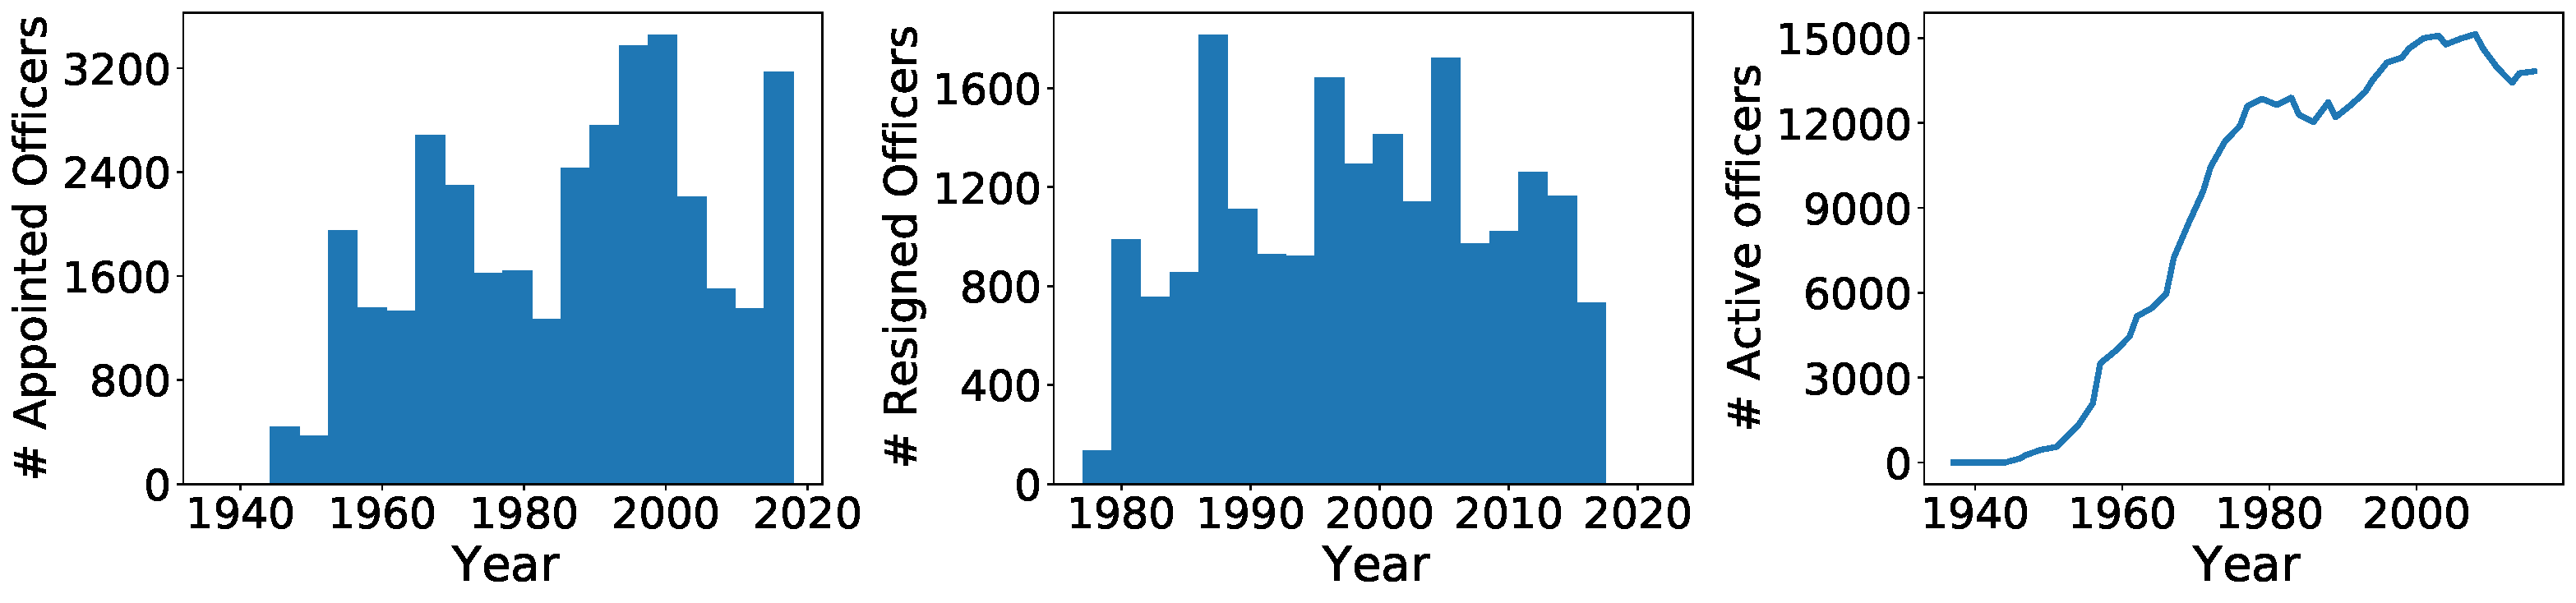
\includegraphics[width=\textwidth]{figs/history} 
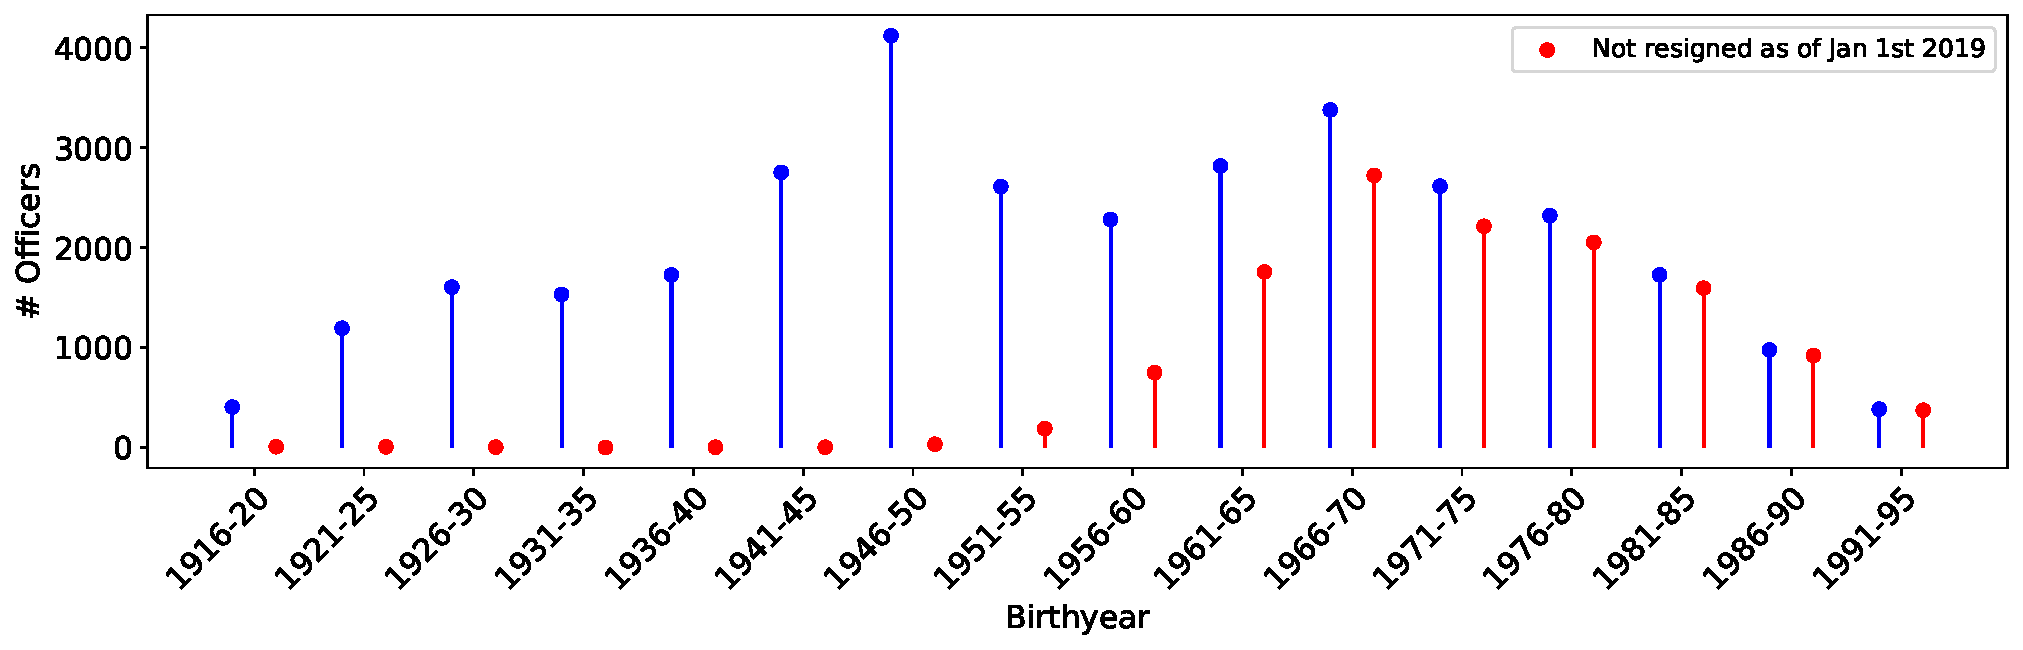
\includegraphics[width=\textwidth]{figs/history_by} 
\caption{Officer birth years (bottom), appointments (top left), resignations (top center), and active
officers (top right) appearing in the CPD roster database from the years 1940 to 2019.}
\label{fig:history}
\end{figure}


\begin{figure}[t!] 
	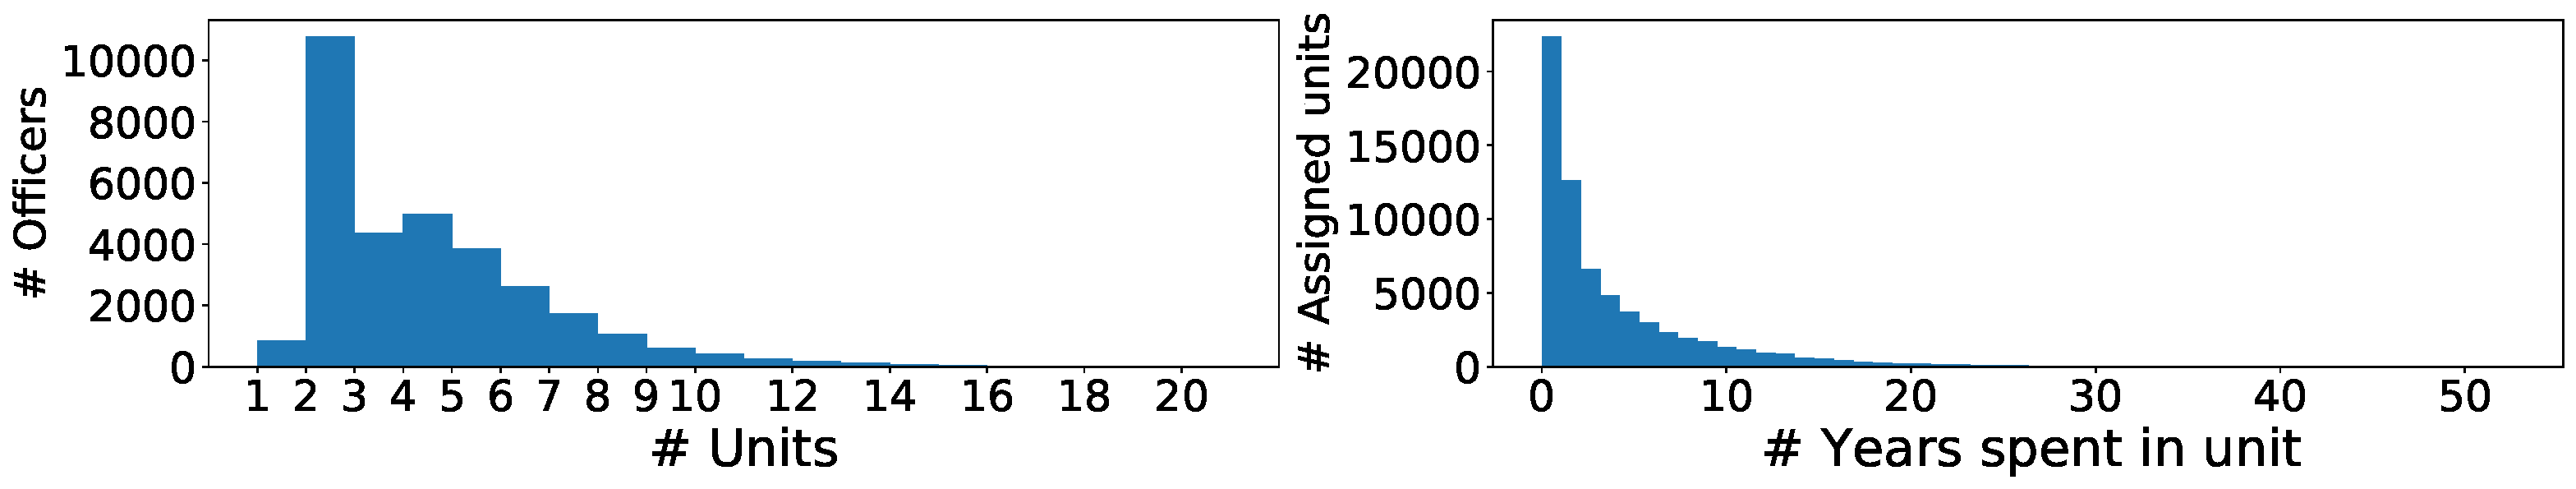
\includegraphics[width=\textwidth]{figs/units_officers.pdf} 
	\caption{Histograms of the number of unit assignments for
officers over their career (left), and the number of years spent in each unit for assignments that had terminated by 2019-01-01 (right).}
\label{fig:units}
\end{figure}

\begin{figure}[t!] 
\begin{subfigure}{0.44\textwidth}
	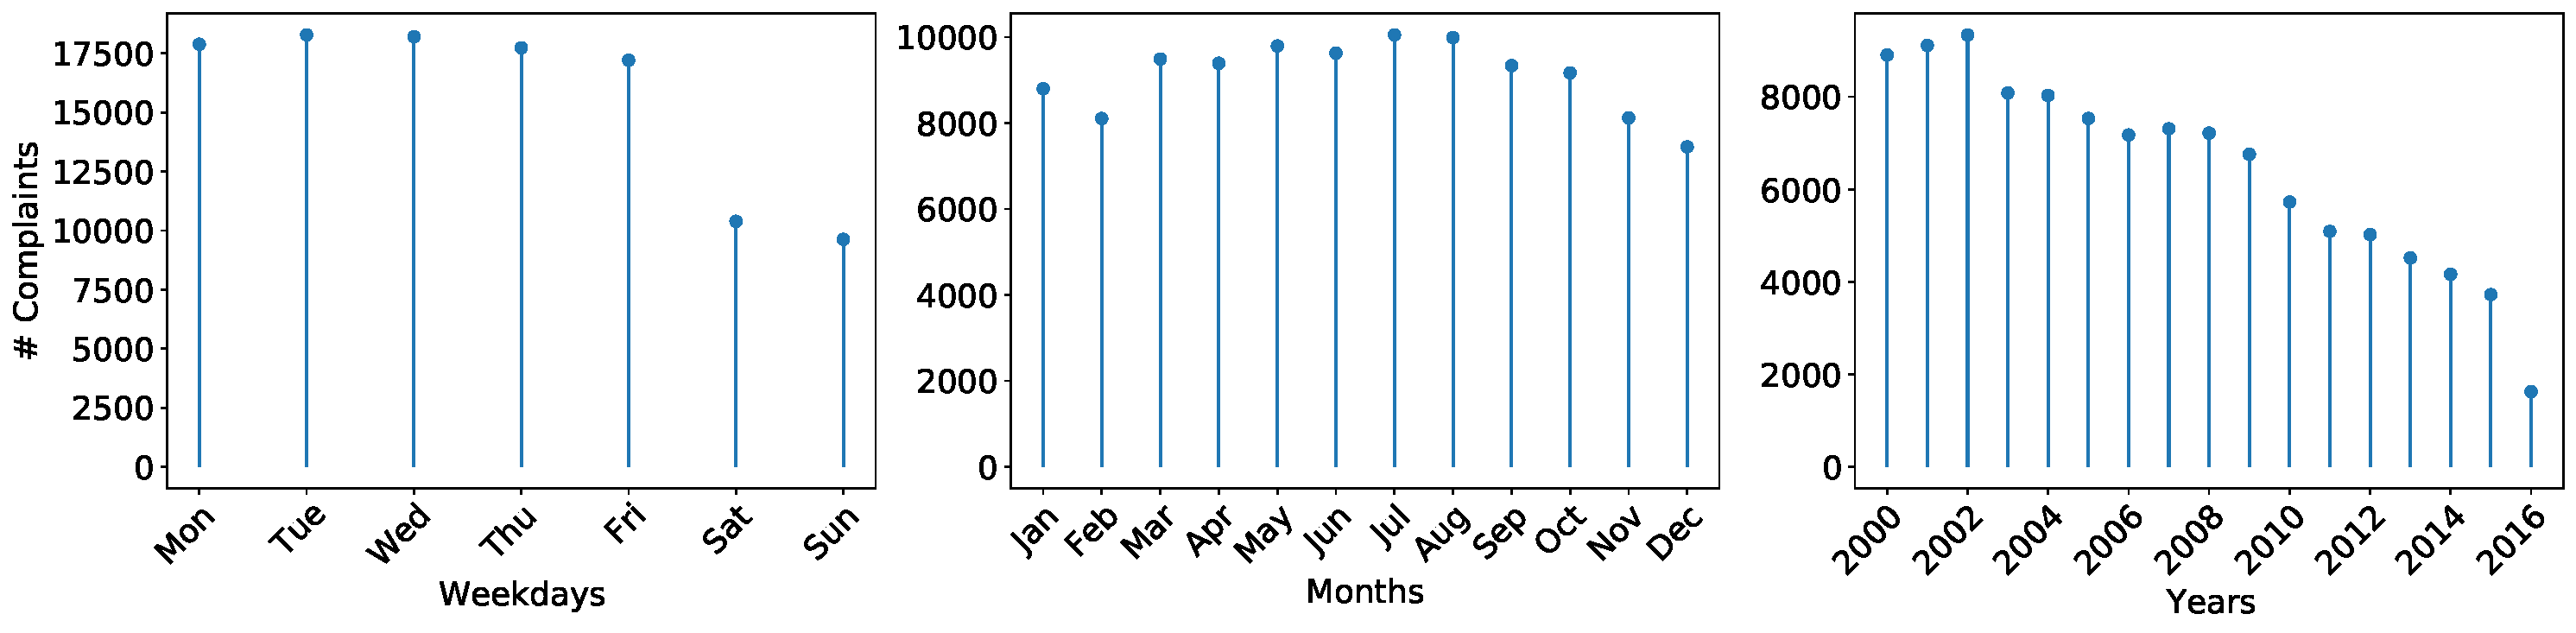
\includegraphics[width=\textwidth, clip, trim= 970 0 0 0]{figs/complaints_times} 
\end{subfigure}
\begin{subfigure}{0.52\textwidth}
	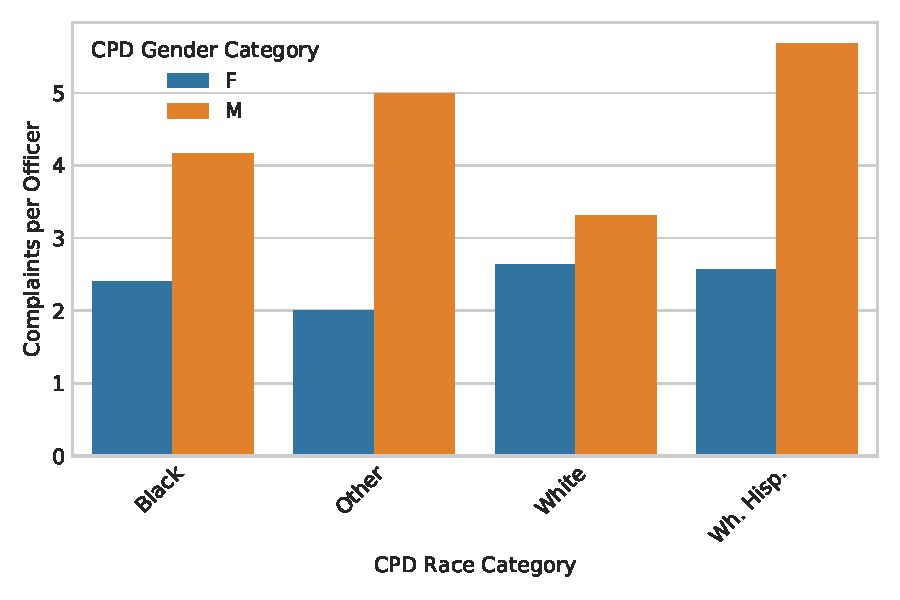
\includegraphics[width=\textwidth]{figs/complaints} 
\end{subfigure}
	\caption{Complaints filed by year (left) and complaints per officer by race and gender (right).} \label{fig:complaints}
\end{figure}
\begin{figure}[t!] 
\begin{subfigure}{0.43\textwidth}
\raisebox{.5cm}{
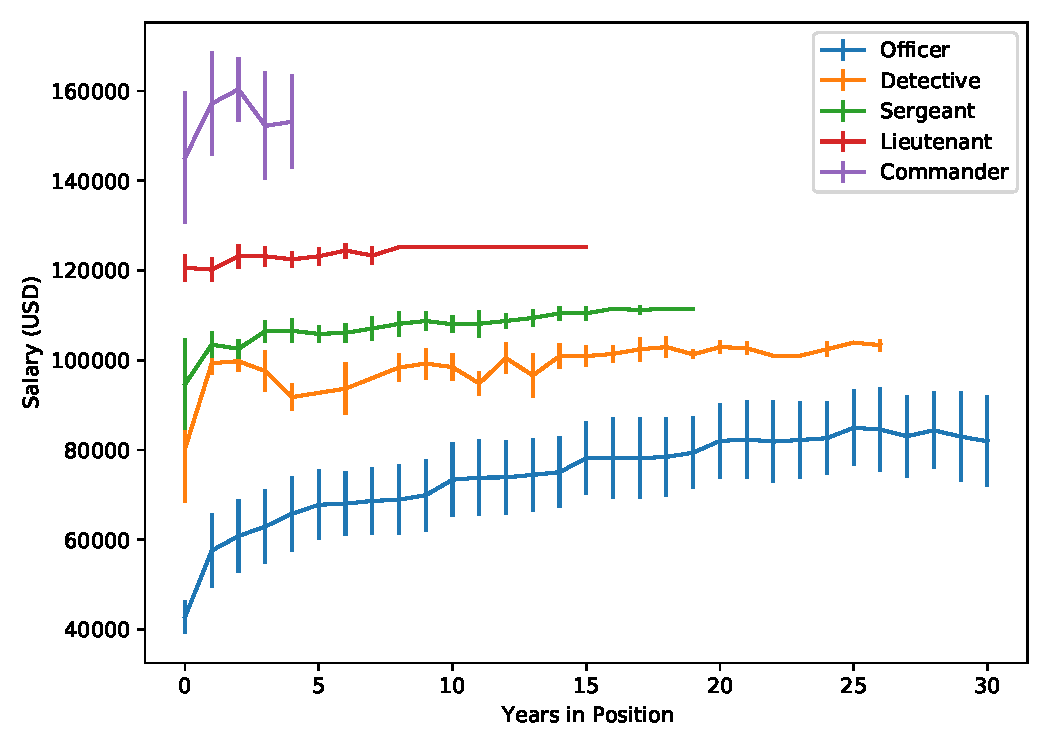
\includegraphics[width=\textwidth]{figs/salary} 
}
\end{subfigure}
\begin{subfigure}{0.53\textwidth}
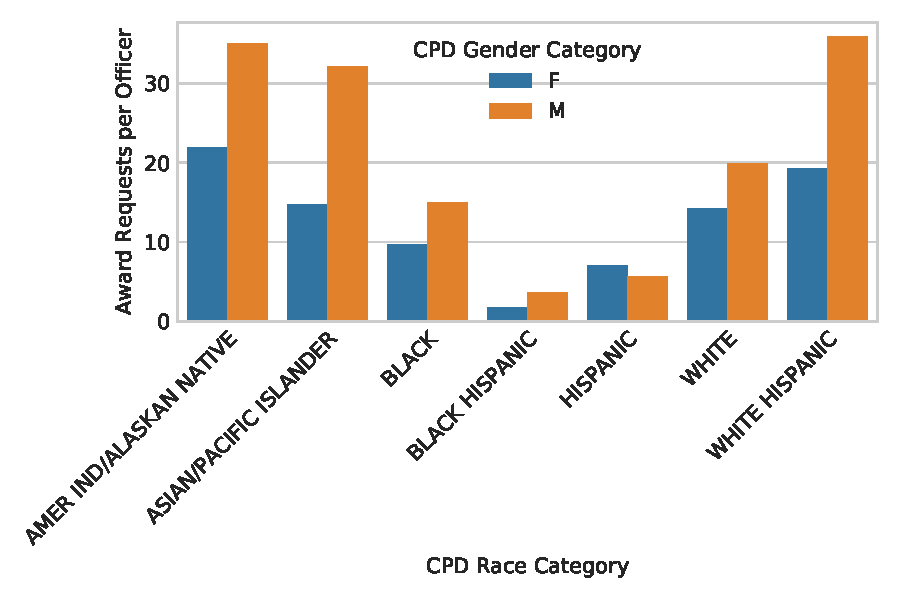
\includegraphics[width=\textwidth]{figs/awards} 
\end{subfigure}
\caption{Officer salaries as a function of the number of years in a selection of representative positions (left),
and the number of award requests per officer by race and gender (right).} \label{fig:salary_awards}
\end{figure}
\begin{figure}[t!] 
	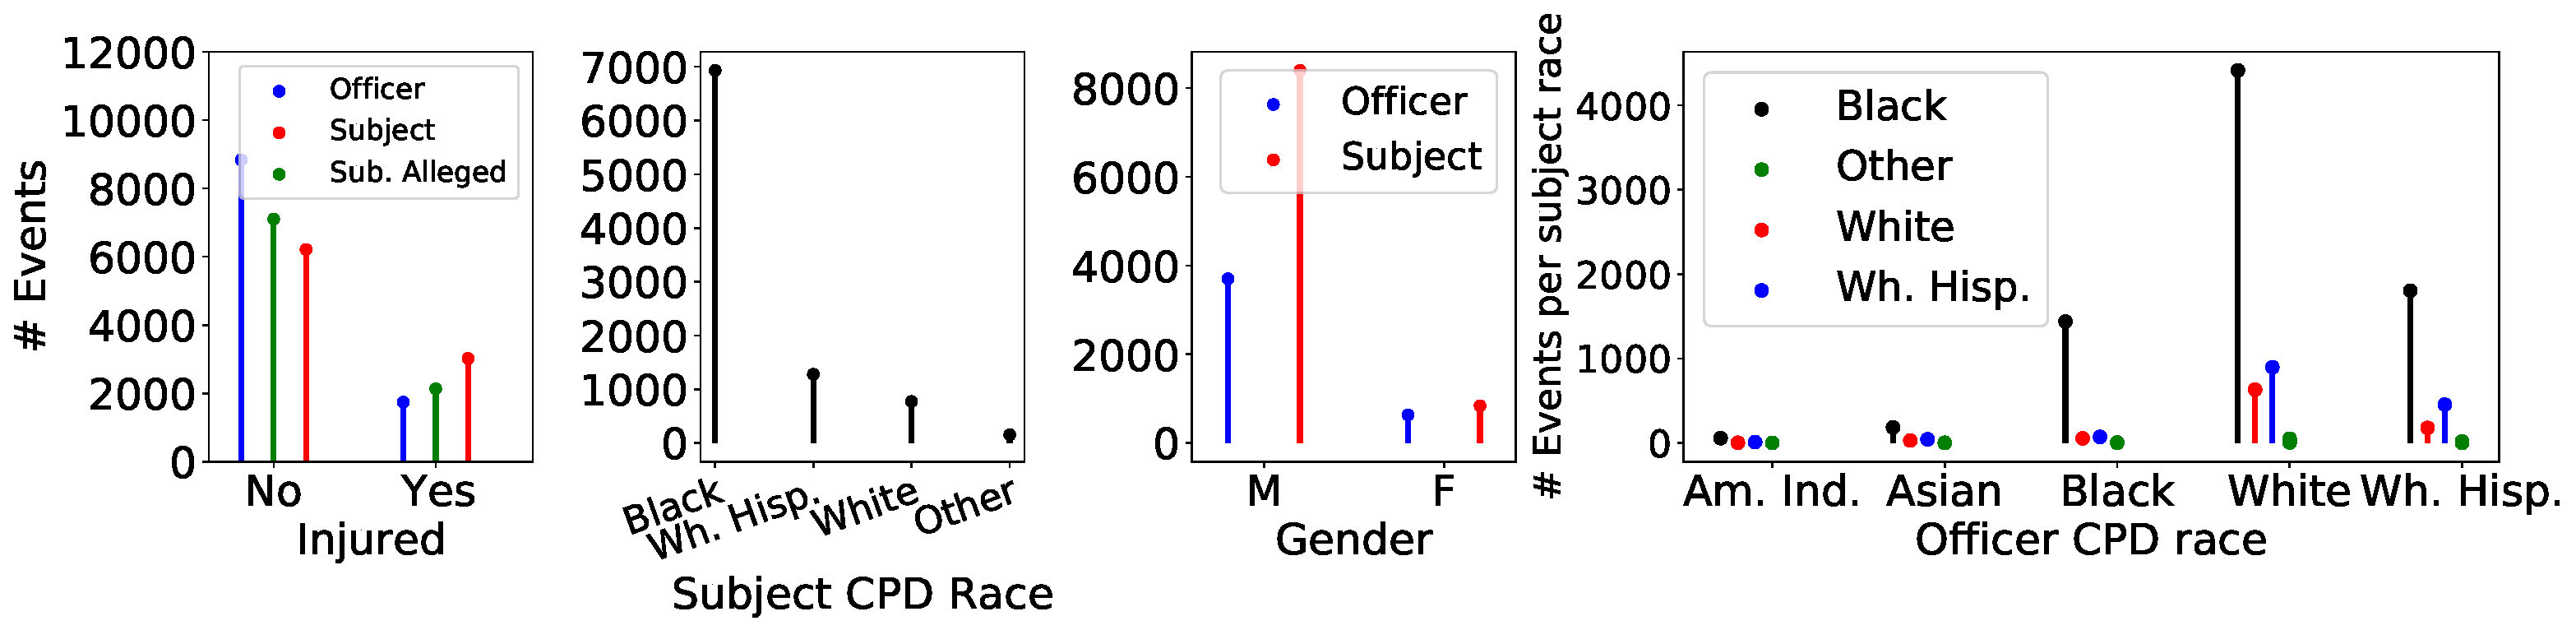
\includegraphics[width=\textwidth]{figs/trr_stats} 
	\caption{Summary counts of TRRs by race, gender, and injury status.} \label{fig:trrs_stats1}
\end{figure}


\paragraph{Complaints.} 
We report in \cref{fig:complaints} patterns of complaints as functions of both time
and officer demographic. This figure highlights another important feature of the data: 
the number of complaints filed gradually reduces over the years, potentially as a 
consequence of the perception of ineffectiveness of such complaints \cite{xx}.
It is also clear in this figure that male officers of color receive proportionally more complaints
than both female officers and white officers, indicating potential racial bias in complaint filings.
Supplemental figures in \cref{sec:additional_figs} demonstrate as well that fewer complaints are 
filed during the weekends and colder months.

\paragraph{Salary and Awards.} \cref{fig:salary_awards} shows officer salary for a small number of representative
positions versus years of experience, as well as the number of award requests filed for officers by demographic.
Unsurprisingly, generally salary increases with experience and with increasing rank. 
And \cref{fig:salary_gender_race} in the appendix shows that salary does not appear to depend strongly on either race or gender,
likely because officers are unionized with strict rules about salary progression.
However, \cref{fig:salary_awards} and \cref{fig:position} both hint that there may be implicit forms of gender
bias present in the data. In particular, awards appear to be requested for male officers at a higher rate than for female officers,
and there is a trend of males disproportionally occupying higher ranks as compared to females.
\cref{fig:position} also indicates that there may be a trend of white officers being promoted more readily 
through the earlier ranks (officer, detective, sergeant) than officers of color.
This trend may not appear at the higher ranks (lieutenant and above), although strong conclusions are difficult without 
rigorous statistical analysis as there are many fewer officers at these ranks.

\paragraph{Tactical Response Reports.}
\cref{fig:trrs_stats1} presents summaries of the tactical response reports in the data.
 In most cases, neither the officers nor the
subjects involved are injured, although civilians get injured at a much higher
rate (left subplot), and officers tend to fire first (4593 instances versus 329).
Analysis involving these data should account for possible racial bias in officer use of force: 
black civilians are the subject of a TRR over 4 times more often than the next 
most frequent subject race. 
\Cref{fig:trrs_times} in the appendix also provides some 
insight into the temporal nature of TRRs: they are filed more frequently 
at night, on the weekends, and during warmer months. 
There is an unusual spike in TRRs betweem 2010-12 that warrants further investigation.


%\begin{tabular}{c|c|c|c|}
%\cline{2-4}
%                                                    & \textit{Member} & \textit{Subject} & \textit{Other} \\ \hline
%\multicolumn{1}{|c|}{\textit{\textbf{Fired first}}} & 4593            & 171               & 158            \\ \hline
%\end{tabular}



